\documentclass[10pt,aspectratio=16:9]{beamer}
\usepackage[utf8]{inputenc}
\usepackage{graphicx}
\usepackage{listings}
\usepackage{xcolor}
\usepackage{booktabs}
\usepackage{tikz}
\usetikzlibrary{shapes,arrows,positioning}

% Color definitions
\definecolor{primaryblue}{RGB}{25, 55, 100}
\definecolor{lightbg}{RGB}{245, 247, 250}
\definecolor{accentgreen}{RGB}{76, 175, 80}
\definecolor{accentred}{RGB}{244, 67, 54}

% Beamer theme customization
\setbeamercolor{palette primary}{bg=primaryblue,fg=white}
\setbeamercolor{frametitle}{bg=primaryblue,fg=white}
\setbeamercolor{background canvas}{bg=white}
\setbeamercolor{normal text}{fg=primaryblue}
\setbeamercolor{block title}{bg=primaryblue,fg=white}
\setbeamercolor{block body}{bg=lightbg,fg=primaryblue}
\setbeamercolor{section in toc}{fg=primaryblue}

% Title page and structure
\setbeamertemplate{title page}{
  \begin{beamercolorbox}[sep=1em,wd=\paperwidth,ht=\paperheight]{palette primary}
    \vfill
    \begin{center}
      {\Large \textbf{\inserttitle}} \\[0.5em]
      {\small \insertsubtitle} \\[1.5em]
      {\footnotesize \insertauthor} \\[0.5em]
      {\footnotesize \insertdate}
    \end{center}
    \vfill
  \end{beamercolorbox}
}

\setbeamertemplate{frametitle}{\vspace{0.3em}\insertframetitle}

\title{ComputerXRobot}
\subtitle{A Benchmark for Learning Robotic Desktop Manipulation}
\author{Anurag Dhiman}
\date{November 2026}

\begin{document}

% ============================================================================
% TITLE SLIDE
% ============================================================================
\begin{frame}[plain]
  \titlepage
\end{frame}

% ============================================================================
% OVERVIEW
% ============================================================================
\begin{frame}{Project Overview}
  \begin{columns}
    \column{0.5\textwidth}
    \begin{itemize}
      \item \textbf{Goal}: Benchmark for learning policies to operate computers
      \item \textbf{Scope}: Desktop interaction (keyboard, mouse, visual feedback)
      \item \textbf{Agent}: 5-DOF robotic arm + finger on MuJoCo 3 simulator
      \item \textbf{Complexity}: 9 tasks × 4 difficulty levels
      \item \textbf{Key Innovation}: Hard tier with realistic hidden dynamics
    \end{itemize}

    \column{0.5\textwidth}
    \begin{center}
      \vspace{0.5em}
      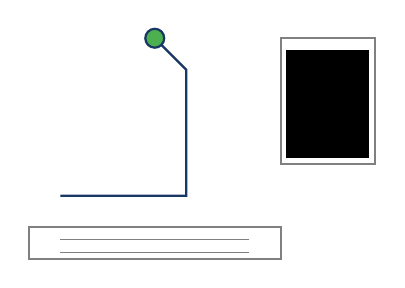
\begin{tikzpicture}[scale=0.8]
        % Arm representation
        \draw[thick, primaryblue] (0,0) -- (2,0) -- (2,2) -- (1.5,2.5);
        \draw[thick, primaryblue, fill=accentgreen] (1.5,2.5) circle (0.15);
        % Keyboard
        \draw[thick, gray] (-0.5,-1) rectangle (3.5,-0.5);
        \draw[gray] (0,-0.9) -- (3,-0.9);
        \draw[gray] (0,-0.7) -- (3,-0.7);
        % Monitor
        \draw[thick, gray] (3.5,0.5) rectangle (5,2.5);
        \draw[fill=black] (3.6,0.6) rectangle (4.9,2.3);
      \end{tikzpicture}
    \end{center}
  \end{columns}
\end{frame}

% ============================================================================
% SECTION 1: PROBLEM & OBJECTIVE
% ============================================================================
\section{Problem \& Objective}

\begin{frame}{Problem: The Computer Control Bottleneck}
  \begin{block}{Challenge}
    \vspace{0.3em}
    Robotic manipulation over long horizons with visual feedback and latency constraints
    \vspace{0.3em}
  \end{block}

  \vspace{1em}

  \begin{columns}
    \column{0.5\textwidth}
    \textbf{Existing Gaps:}
    \begin{itemize}
      \item Limited benchmarks for desktop interaction tasks
      \item Lack of standardized evaluation protocols
      \item Mismatch between sim and real control latency
      \item No generalization metrics for unseen dynamics
    \end{itemize}

    \column{0.5\textwidth}
    \textbf{Our Objective:}
    \begin{itemize}
      \item Establish a reproducible benchmark
      \item Test policy robustness to dynamics variation
      \item Compare behavior cloning vs.\ adaptive control
      \item Enable research on sim-to-real transfer
    \end{itemize}
  \end{columns}
\end{frame}

% ============================================================================
% SECTION 2: SYSTEM ARCHITECTURE
% ============================================================================
\section{System Architecture}

\begin{frame}{High-Level Pipeline}
  \begin{center}
    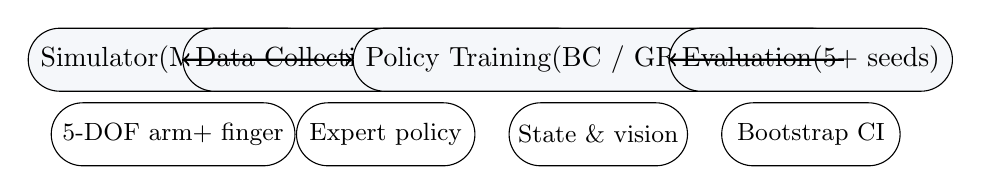
\begin{tikzpicture}[scale=0.9, every node/.style={draw, rounded rectangle, minimum height=0.8cm, minimum width=2.5cm}]
      \node[fill=lightbg] (env) at (0,0) {Simulator\\(MuJoCo 3)};
      \node[fill=lightbg] (data) at (3,0) {Data Collection\\(Oracle Demos)};
      \node[fill=lightbg] (train) at (6,0) {Policy Training\\(BC / GRU / DAgger)};
      \node[fill=lightbg] (eval) at (9,0) {Evaluation\\(5+ seeds)};

      \draw[->,thick] (env) -- (data);
      \draw[->,thick] (data) -- (train);
      \draw[->,thick] (train) -- (eval);

      % Add descriptors
      \node[anchor=north, font=\small] at (0,-0.6) {5-DOF arm\\+ finger};
      \node[anchor=north, font=\small] at (3,-0.6) {Expert policy};
      \node[anchor=north, font=\small] at (6,-0.6) {State \& vision};
      \node[anchor=north, font=\small] at (9,-0.6) {Bootstrap CI};
    \end{tikzpicture}
  \end{center}

  \vspace{1.5em}

  \begin{columns}
    \column{0.5\textwidth}
    \textbf{Environment:}
    \begin{itemize}
      \item Keyboard \& mouse control
      \item 50 Hz control loop
      \item 4 camera views
      \item Realistic physics simulation
    \end{itemize}

    \column{0.5\textwidth}
    \textbf{Tasks:}
    \begin{itemize}
      \item 9 desktop interaction tasks
      \item Standard splits: test, val, visual, dynamics
      \item Hard tier: realistic hidden dynamics
      \item Latency: 0–80 ms (action delay)
    \end{itemize}
  \end{columns}
\end{frame}

% ============================================================================
% SECTION 3: MODEL & ALGORITHMS
% ============================================================================
\section{Model \& Algorithms}

\begin{frame}{Policy Learning Approaches}
  \vspace{-0.5em}
  \begin{table}
    \footnotesize
    \centering
    \begin{tabular}{l|c|c|c}
      \toprule
      \textbf{Method} & \textbf{Architecture} & \textbf{Training} & \textbf{Privileged?} \\
      \midrule
      Oracle & Scripted & — & \checkmark \\
      BC & MLP encoder & 1 round & — \\
      BC-History & MLP + 4-step history & 1 round & — \\
      \textbf{BC-GRU} & \textbf{MLP + GRU(256)} & \textbf{60 epochs} & \textbf{—} \\
      Adaptive-Expert & GRU + online ID & Online & — \\
      BC-DAgger & MLP + data aggregation & 2 rounds & — \\
      \textbf{BC-GRU-DAgger} & \textbf{GRU + aggregation} & \textbf{2 rounds} & \textbf{—} \\
      \bottomrule
    \end{tabular}
  \end{table}

  \vspace{0.8em}

  \begin{block}{Key Innovation: Recurrent Behavior Cloning}
    \vspace{0.2em}
    \textbf{BC-GRU}: Encoder $\to$ GRU(256) over episode history $\to$ output head on [encoding, hidden state]
    \begin{itemize}
      \item Truncated BPTT with chunk size 128
      \item 8 episodes/batch, AdamW lr 1e-3 cosine schedule
      \item Smooth-L1 loss (β=0.05), finger action weight 4×
    \end{itemize}
    \vspace{0.2em}
  \end{block}
\end{frame}

\begin{frame}{DAgger: Online Data Aggregation}
  \begin{columns}
    \column{0.5\textwidth}
    \textbf{Algorithm (Ross et al., 2011):}
    \begin{enumerate}
      \item Train student on oracle demos
      \item Play 25 episodes/task (all splits)
      \item Oracle labels all visited states
      \item Aggregate data, retrain student
      \item Repeat (2 iterations)
    \end{enumerate}

    \column{0.5\textwidth}
    \textbf{Why DAgger?}
    \begin{itemize}
      \item Addresses distribution shift
      \item Student learns from failures
      \item Recovers policy collapse
      \item Works for any learner (BC, GRU, etc.)
    \end{itemize}
  \end{columns}

  \vspace{0.8em}

  \begin{alertblock}{Key Result}
    \centering
    \textbf{BC-GRU-DAgger}: 98.8\% success [96.9, 99.9] with stable performance across all 5 seeds.
  \end{alertblock}
\end{frame}

% ============================================================================
% SECTION 4: DATA PIPELINE & TRAINING
% ============================================================================
\section{Data Pipeline \& Training}

\begin{frame}{Data Collection \& Preprocessing}
  \begin{columns}
    \column{0.5\textwidth}
    \textbf{Oracle Demonstrations:}
    \begin{itemize}
      \item 100 demos per task
      \item 9 tasks × 2 splits (train, aux) = 1800 episodes
      \item State features: joint angles, velocities, button presses
      \item Vision: 84×84 RGB from 4 cameras
      \item $\sim$89k total samples (state) or 540k (vision)
    \end{itemize}

    \column{0.5\textwidth}
    \textbf{Training Setup:}
    \begin{itemize}
      \item Batch size: 8 episodes
      \item Epochs: 60 (state), 30 (vision)
      \item Optimizer: AdamW (lr 1e-3)
      \item Learning rate schedule: cosine annealing
      \item Validation: held-out episodes
    \end{itemize}
  \end{columns}

  \vspace{1em}

  \begin{block}{Hard Tier: Realistic Hidden Dynamics}
    \vspace{0.2em}
    Per-episode randomization (5–20 seeds):
    \begin{itemize}
      \item Control latency: 0–80 ms (action delay steps)
      \item Arm sag, actuation noise, observation noise
      \item Per-key spring force, double-click timing, auto-repeat
      \item Mouse acceleration, pointer rotation
    \end{itemize}
    \vspace{0.2em}
  \end{block}
\end{frame}

% ============================================================================
% SECTION 5: EVALUATION & BENCHMARKS
% ============================================================================
\section{Evaluation \& Benchmarks}

\begin{frame}{Evaluation Metrics \& Statistics}
  \vspace{-0.5em}
  \begin{block}{Bootstrap Cross-Validation (Agarwal et al., 2021)}
    \vspace{0.2em}
    \begin{itemize}
      \item 2000 bootstrap resamples (seeds with replacement)
      \item 95\% confidence intervals over (seed, task) success rates
      \item IQM (Interquartile Mean): 25\% trimmed mean for robust aggregation
      \item Paired comparisons: $P(\text{Agent A} > \text{Agent B})$
    \end{itemize}
    \vspace{0.2em}
  \end{block}

  \vspace{0.8em}

  \begin{table}
    \footnotesize
    \centering
    \begin{tabular}{l|c|c|c}
      \toprule
      \textbf{Agent} & \textbf{Range} & \textbf{Mean} & \textbf{Seeds} \\
      \midrule
      Oracle & 99.4 [98.3, 100.0] & — & 5 \\
      BC & 70.2 [60.0, 79.9] & 69.8 & 5 \\
      BC-History & 78.4 [68.7, 88.0] & 78.1 & 5 \\
      \textbf{BC-GRU-DAgger} & \textbf{98.8 [96.9, 99.9]} & \textbf{98.8} & \textbf{5} \\
      Adaptive-Expert & 99.4 [98.3, 100.0] & — & 5 \\
      \bottomrule
    \end{tabular}
  \end{table}

  \vspace{0.5em}

  \textbf{All 5 seeds}: Reproducibility verified, no git-dirty flags.
\end{frame}

\begin{frame}{Generalization: Hard Tier Results}
  \vspace{-0.5em}
  \begin{columns}
    \column{0.5\textwidth}
    \textbf{Latency Robustness:}
    \begin{itemize}
      \item Control delay (0–80 ms) causes policy collapse
      \item Adaptive-Expert: 99.4\% (online ID)
      \item BC-GRU-DAgger: 20.9\% (learned only)
      \item Mismatch between train latency and test dynamics
    \end{itemize}

    \column{0.5\textwidth}
    \textbf{Memory Scaling:}
    \begin{itemize}
      \item 4-step history marginal benefit: Δ 7.0 [−22, 32.8]
      \item GRU helps within-distribution but not OOD
      \item Learned models cannot adapt to new latencies
    \end{itemize}
  \end{columns}

  \vspace{1em}

  \begin{alertblock}{Key Finding}
    Latency is the primary generalization bottleneck. Adaptive online identification (like
    Adaptive-Expert) is essential for handling unseen dynamics.
  \end{alertblock}
\end{frame}

% ============================================================================
% SECTION 6: DEPLOYMENT & SCALABILITY
% ============================================================================
\section{Deployment \& Scalability}

\begin{frame}{Infrastructure \& Reproducibility}
  \begin{columns}
    \column{0.5\textwidth}
    \textbf{Local Development (CPU):}
    \begin{itemize}
      \item State-track results: $\sim$1 day on MacBook Air
      \item 5 seeds, all agents, ablation
      \item Standard splits + hard tier
      \item Reproducible via \texttt{run\_cpu.sh}
    \end{itemize}

    \column{0.5\textwidth}
    \textbf{GPU Scaling (A100):}
    \begin{itemize}
      \item Vision-track training: $\sim$1 hour per model
      \item Docker + EGL headless rendering
      \item Parallelized eval (32 workers)
      \item Fully automated via \texttt{run\_gpu.sh}
    \end{itemize}
  \end{columns}

  \vspace{1em}

  \begin{block}{Packaging \& Distribution}
    \vspace{0.2em}
    \begin{itemize}
      \item PyPI package: \texttt{pip install -e .}
      \item Git commit tracking: \texttt{meta.git\_commit}, \texttt{meta.git\_dirty}
      \item Reproducible environments: \texttt{environment.yml}, \texttt{Dockerfile}
      \item Open source: \url{github.com/Anurag9Dhiman/ComputerXRobot}
    \end{itemize}
    \vspace{0.2em}
  \end{block}
\end{frame}

% ============================================================================
% SECTION 7: CHALLENGES & NEXT STEPS
% ============================================================================
\section{Challenges \& Next Steps}

\begin{frame}{Technical Challenges Addressed}
  \begin{columns}
    \column{0.5\textwidth}
    \textbf{Solved:}
    \begin{itemize}
      \item Memory in BC: GRU enables state tracking
      \item Policy collapse: DAgger recovery verified
      \item Variance: Bootstrap statistics across seeds
      \item Reproducibility: Git commit tracking in results
    \end{itemize}

    \column{0.5\textwidth}
    \textbf{Remaining Open:}
    \begin{itemize}
      \item Vision-based control precision
      \item Generalization to real latency distributions
      \item Multi-agent coordination
      \item Failure mode analysis \& recovery
    \end{itemize}
  \end{columns}

  \vspace{1em}

  \begin{alertblock}{Next Steps (Roadmap)}
    \begin{enumerate}
      \item Vision-track baseline on A100 (3 seeds, state-of-art vision encoders)
      \item Dynamics prediction models (world models)
      \item Sim-to-real transfer protocols
      \item Scaling to multi-agent scenarios
    \end{enumerate}
  \end{alertblock}
\end{frame}

\begin{frame}{Open Research Questions}
  \begin{enumerate}
    \item How much latency robustness can learned policies achieve with better domain randomization?
    \item Does vision-based control enable better generalization than state-only?
    \item Can we learn latency-aware policies without online adaptation?
    \item What is the sample complexity for reliable transfer to real hardware?
  \end{enumerate}

  \vspace{1.5em}

  \begin{block}{Impact}
    \vspace{0.2em}
    \textbf{ComputerXRobot} establishes a standard benchmark for desktop manipulation with
    rigorous evaluation methodology, enabling reproducible research on robustness, generalization,
    and adaptation in long-horizon robotic tasks.
    \vspace{0.2em}
  \end{block}
\end{frame}

% ============================================================================
% CLOSING SLIDE
% ============================================================================
\begin{frame}[plain]
  \begin{beamercolorbox}[sep=1em,wd=\paperwidth,ht=\paperheight]{palette primary}
    \vfill
    \begin{center}
      {\Large \textbf{Thank You}} \\[1em]
      {\normalsize Questions \& Discussion}
    \end{center}
    \vfill
  \end{beamercolorbox}
\end{frame}

\end{document}
